\chapter{Theory}
\label{chapter:theory}

% {{{1 MEAN CURVATURE FLOW
\section{Mean Curvature Flow}

Given a family of hypersurfaces $ S_t $ of $ \R^d $ given by $ x(u) $, we say
that $ S_t $ is evolving by mean curvature if it satisfies the following
equation:

$$ \partiald{x(u)}{t} = \vec{\kappa}(u) $$

Where $ \vec{\kappa}(u) $ is the mean curvature vector of $ S_t $ at $ u $ and
$ \partiald{x(u)}{t} $ is the normal velocity at $ u $.

Put in more simple words, it says that at each step we move each point of the
hypersurface $ S_t $ in the direction of the inward normal by an amount given by
the mean curvature.

Now, we will prove that the mean curvature flow belongs to a more general
category of geometric flows: the gradient flows. Given an energy $ f $, we say
that $ S $ evolves according to the gradient flow of $ f $ if we have:

$$ \partiald{x}{t} = \nabla f(x) $$

Indeed, the next proposition shows the relation between the mean curvature flow
and the area functional.

\begin{proposition}
    The mean curvature flow is the gradient flow of the area functional.
\end{proposition}

To prove this proposition, we will need some background on hypersurfaces.

First, the notion of the reach of an hypersurface: it is widely used in
computational geometry.
\begin{definition}
    The reach of a manifold $ M $ denoted by $ reach(M) $ is the largest $ r
    \geq 0 $ for which for any $ p \in M^r $, there exists a unique $ q \in M $
    such that $ q = p_M(p) $ where $ p_M $ is the projection on $ M $. $ p_M(x)
    $ is defined such that $ || x - p_M(x) || = d(x, M) $.
\end{definition}

The reach has some interesting properties (see \cite{merigot2009detection} for a
more detailed study):

\begin{itemize}
    \item For example, if we consider a circle in the plane of radius $ R $,
        then every point in the plane has a unique projection on the circle
        except the center which is at distance $ R $ of every point on the
        circle: there is no closest point.  Consequently, its reach is $ R $.

    \item Another more general example is that any convex set has infinite
        reach. This is because the projection on a closed convex set is always
        uniquely defined.

    \item The reach is also related to the Local Feature Size (LFS) defined in
        \cite{amenta1999surface}: $ LFS(p) = d(p, \mathcal{M}) $ $ reach(M) =
        \min\limits_{p \in M}~LFS(p) $ where $ \mathcal{M}  $ is the medial axis
        of $ M $.

    \item The reach is also always upper bounded by the minimum radius of
        curvature. There are no results on the lower bound. Indeed, consider the
        following example: two spheres of radius $ R $ at distance $ \epsilon $,
        then the radius of curvature is always $ R $ but the reach of the union
        if $ \frac{\epsilon}{2} $.
\end{itemize}

Then, some facts about the curvature of embedded hypersurfaces:

\begin{proposition}
    For an hypersurface $ S \subseteq \R^d $, the map $ x \in S \rightarrow
    \vec{n}_S(x) $ where $ \vec{n}_S(x) $ is the normal vector of $ S $ at $ x $ is
    called the Gauss map while its derivative is called the shape operator.

    Then, we have that the shape operator is diagonalizable and its eigenvalues
    are the $ d-1 $ principal curvatures at $ x $: $ \kappa_1(x), \ldots,
    \kappa_{d-1}(x) $.

    We will also denote by $ \vec{\kappa}(x) $ the mean curvature vector at $ x
    $: $ \vec{\kappa}(x) = \sum_{i=1}^{d-1} \kappa_i(x) \vec{n}_S(x) $.
    \label{prop:curvatures-surface}
\end{proposition}

And finally, a change of variable result:

\begin{lemma}
    \label{lemma:diffeo}
    Given a smooth hypersurface $ S $, and a function $ f : S \times [0, r] \to \R^d $
    defined by $ f(x, t) = x + t \phi(x) \vec{n}_S(x) $ where $ \phi : \R^d \to
    \R^d $ is a smooth vector field then $ f $ is a diffeomorphism for $ r < reach(S) $.

    If we decompose this substitution on $ T_p(S) \times [-r, r] $, where $ T_p(S)
    $ is the tangent space of $ S $ at $ p $, we get: $ D \phi = id + r D
    \vec{n_S}(q) $.  So, its Jacobian is given by: $ J_f(x) = \det(id + t \phi(x) D
    \vec{n}_S (x)) $.

    Using the previous proposition, we get:
    $$ J_f(x) = \prod_{i=1}^{d-1} (1 + t \phi(x) \kappa_i(x)) $$
\end{lemma}

We will denote by $ Vol^d(S) $ the $d$-dimensional volume of an object $ S
$.

Then, we can tackle the proof:

\begin{proof}
    We parametrize the evolving surface $ S_t $ by $ S_t = \{ x + t \phi(x)
    \vec{n}(x), x \in S_0\} $ where $ \phi : \R^d \rightarrow \R^d $ is a smooth
    vector field. We denote by $ A = Vol^{d-1} $ the area functional.
    Then, we have, using the lemma \ref{lemma:diffeo}:
    \begin{align*}
        Vol^{d-1}(S_t) &= \int_{S_t} 1 dx = \int_{S_0} J_{\phi}(x) dx \\
        &= \int_{S_0} \prod_{i=1}^{d-1} (1 + t \phi(x) \kappa_i(x)) \\
        &= \int_{S_0} 1dx + t \int_{S_0} \phi(x) \vec{\kappa}(x) dx + O(t^2)
    \end{align*}

    So:
    $$ \lim\limits_{t \to 0} \frac{A(S_t) - A(S_0)}{t}= \int_{S_0}
    \phi(x) \vec{\kappa}(x) dx $$

    This equation tells us exactly that if we perturbate a surface by $ \phi $
    then the variation of the area functional is linked to the mean curvature.
\end{proof}

This proposition will be at the basis of our work. We will replace "hypersurface"
with "point cloud sampled on an hypersurface" and try to approximate the area of
the hypersurface by something which can be computed using only the point cloud.

% {{{1 DISCRETIZATION OF THE AREA
\section{Discretization of the area}

In this section, we will try to compute an approximation of the area of an
hypersurface with only knowing points sampled on it.

First, we will introduce the $r$-offset of a point cloud:

\begin{definition}
    For $ r > 0 $ and a point cloud $ P $, we define the $r$-offset of $ P $
    denoted by $ P^r $ by:
    $$ P^r = \bigcup_{p \in P} B(p, r)$$
\end{definition}

It can also be seen as the Minkowski sum of $ P $ and the euclidean ball $ B(0,
r) $.

\begin{definition}
    For any sets $ A $ and $ B $ of a vector space, we define the Minkowski sum
    of $ A $ and $ B $ denoted by $ A \oplus B $:
    $$ A \oplus B = \{ a + b, a \in A, b \in B \} $$
    \label{def:minkowski-sum}
\end{definition}

Then, we will define a similar notion for hypersurfaces called the tubular
neighbourhood:

\begin{definition}
    For any $ r > 0 $, the tubular neighbourhood of an hypersurface $ S $
    denoted by $ S^r $ is defined in the same way as for point clouds:
    $$ S^r = \bigcup_{x \in S} B(x, r) $$
\end{definition}

Using these notions, we can relate the area of an hypersurface to the volume of
its tubular neighbourhood using a variant of the tube formula \cite{weyl1939volume}.

\begin{proposition}
    \label{prop:comp-offset-area}
    If $ S $ is a smooth hypersurface whose reach is positive and $ reach(S) > r
    > 0 $, then: $$ Vol^{d-1}(S) = \frac{Vol^d(S^r)}{2r} + O(r^2) $$

    The constants in the error term of the development only depend on the curvature
    of $ S $.
\end{proposition}

\begin{proof}
    We have: $ Vol^d(S^r) = \int_{S^r} 1 dx $. Now, we will do the following
    change of variable: $ f : S \times [-r, r] \rightarrow S^r $ where $ f(x, t)
    = x + t \vec{n}_K(x) $. Using this substitution and lemma \ref{lemma:diffeo}
    with $ \phi = 1 $:

    \begin{align*}
        Vol^d(S^r) &= \int_S \int_{-r}^r J_f(p) dt dp \\
        &= \int_S \int_{-r}^r \prod_{i=1}^{d-1} (1 + t \kappa_i(p)) dt dp \\
        &= \int_S \int_{-r}^r \left( 1 + \sum_{k=1}^{d-1} t^k \sum_{i_1 < \ldots
                < i_k} \kappa_{i_1}(p) \ldots \kappa_{i_k}(p) \right) dt dp \\
        &= 2r \int_S 1 dp + \int_K \int_{-r}^r \sum_{k=1}^{d-1} t^k \sum_{i_1 < \ldots < i_k} \kappa_{i_1}(p) \ldots \kappa_{i_k}(p) dt dp \\
        &= 2r Vol^{d-1}(S) + O(r^2)
    \end{align*}

    So: $ \frac{Vol^d(S^r)}{2r} = Vol^{d-1}(S) + O(r^2) $.
\end{proof}

This proposition is related to the Minkowski content. It is used to measure the
area of the boundary of a set: the $ d-1 $ dimensional volume in dimension $ d
$.

It is defined as follows:
$$ \lim\limits_{\epsilon \to 0} \frac{\mu(S^{\epsilon}) - \mu(S)}{\epsilon} $$

This is exactly what we computed: a Taylor expansion of $ Vol^d(S^r) $.

Next, we want to approximate $ Vol^d(S^r) $ by $ Vol^d(P^r) $ where $ P \subset
S $ is a point cloud. We will need a formalization of the notion of sampling:

\begin{definition}
    A set of points $ p_i $ is said to be an $\epsilon$-sampling of a manifold $
    M $ if the set of the balls  $ B(p_i, \epsilon) $ verifies: $ M \subseteq
    \bigcup_i B(p_i, \epsilon) $ (see \cite{amenta1999surface}).
\end{definition}

The following proposition bounds the error of this approximation:

\begin{proposition}
    \label{prop:comp-vol-offsets}
    For an hypersurface $ S $ with positive reach and an $\epsilon$-sampling $ P
    \subseteq S $, we have:
    $$ 0 \leq Vol^d(S^r) - Vol^d(P^r) \leq \frac{\epsilon^2}{r} Vol^{d-1}(S) +
    O(\frac{\epsilon^4}{r^2}) $$
\end{proposition}

\begin{proof}
    Since $ P \subseteq S $, then $ Vol^d(S^r) \leq Vol^d(P^r) $.

    Then, we parametrize $ P^r $ by $ f : S \rightarrow P^r $ where $ f(x) = x +
    r(x) \vec{n}_S(x) $ for $ r(x) \in [0, r] $ (see
    \ref{fig:offset-parametrization}).

    \begin{figure}[h]
        \centering
        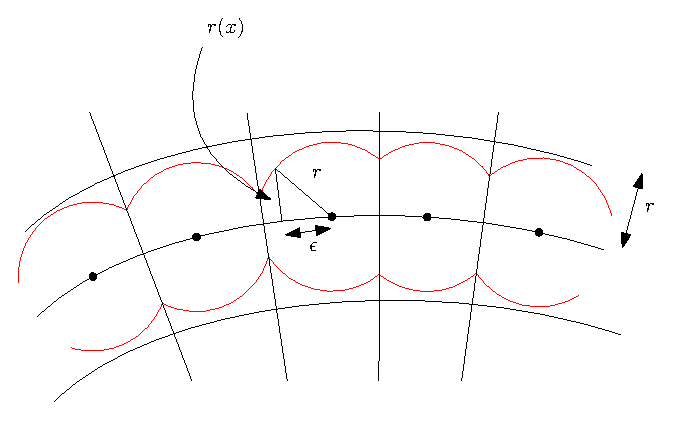
\includegraphics[scale=0.8]{offset-parametrization}
        \caption{Parametrization of the offset (in red)}
        \label{fig:offset-parametrization}
    \end{figure}

    We have:
    \begin{align*}
        r(x)^2 + \epsilon^2 = r^2 \iff& (r - r(x)) (r + r(x)) = \epsilon^2 \\
        \iff& r - r(x) = \frac{\epsilon^2}{r + r(x)} \leq \frac{\epsilon^2}{r} \\
    \end{align*}

    Now, we will use the same formula as in the previous proofs:

    \begin{align*}
        Vol^d(S^r) - Vol^d(P^r) &= \int_{S^r \textbackslash P^r} 1 dp \\
        &= \int_S \int_{r(x)}^r \det(id + t D \vec{n}_S(p)) dt dp \\
        &= \int_S \int_{r(x)}^r \left( 1 + \sum_{k=1}^{d-1} t^k \sum_{i_1 < \ldots
                < i_k} \kappa_{i_1}(p) \ldots \kappa_{i_k}(p) \right) dt dp \\
        &= \int_S (r - r(x)) dp + O((r - r(x))^2) \\
        &\leq \frac{\epsilon^2}{r} Vol^{d-1}(S) + O(\frac{\epsilon^4}{r^2})
    \end{align*}
\end{proof}

Now, combining the previous propositions, we will show that we can approximate
the area of $ S $ by the volume of $ P^r $:

\begin{proposition}
    \label{prop:approx-volume-area}
    Given an hypersurface $ S $, an $\epsilon$-sampling of $ S $: $ P $, we
    have:
    $$ | \frac{Vol^d(P^r)}{2r} - Vol^{d-1}(S) | \leq \frac{\epsilon^2}{2r^2} +
    O(\frac{\epsilon^4}{r^3}) + O(r^2) $$

    So, when $ \frac{\epsilon}{r} $ and $ r $ vanish then $
    \frac{Vol^d(P^r)}{2r} $ converges towards the area of $ S $.
\end{proposition}

\begin{proof}
    We will use the propositions \ref{prop:comp-vol-offsets} and
    \ref{prop:comp-offset-area}.

    We have, using the triangle inequaltiy:
    \begin{align*}
        \left| \frac{Vol^d(P^r)}{2r} - Vol^{d-1}(S) \right| \leq& \left| \frac{Vol^d(P^r)}{2r} -
            \frac{Vol^d(S^r)}{2r} \right| + \left| \frac{Vol^d(S^r)}{2r} -
            Vol^{d-1}(S) \right| \\
        \leq& \frac{\epsilon^2}{2r^2} Vol^{d-1}(S) + O(\frac{\epsilon^4}{r^3}) + O(r^2) \\
    \end{align*}
\end{proof}

At this point, we have shown a way to approximate the area of an hypersurface
with a quantity proportional to the volume of the $r$-offset of a point cloud
sampled on the surface.
Now, we want to study the gradient of this newly computed quantity.

% {{{1 CONVERGENCE OF THE GRADIENT
\section{Convergence of the gradient}

In this section, we will derive formulae for the gradients of the volume of
union of balls in $ \R^d $.

First, we will define what we mean by "gradients":

\begin{definition}
    If $ F : \R^d \times \ldots \times \R^d \to \R $ is a function over
    $d$-dimensional point clouds, then we define $ \nabla_{p_i} F \in \R^d $ by:

    $$ \lim\limits_{\epsilon \to 0} \frac{F(p_1, \ldots, p_{i-1}, p_i + \epsilon
        \delta p_i, p_{i+1}, \ldots, p_N) - F(p_1, \ldots, p_N)}{\epsilon} $$

    In other words, $ \nabla_{p_i} F $ represents the variation of $ F $ if
    we move the ith point by an amount $ \delta p_i $.
\end{definition}

The next proposition gives the gradient of the volume of union of balls :
\begin{proposition}
    Given an hypersurface $ S $ of $ \R^d $ and points sampled on it: $ (p_i) $.
    Then, if we denote by $ A $ the volume of the union of balls, we are
    interested in computing the gradients (defined previously) of $ A $.

    We have:
    \begin{equation}
        \label{eqn:gradient_area_2d}
        \nabla_{p_i} A = \int_{B} \frac{x - p_i}{||x - p_i||} dx
    \end{equation}
    where $ B = \partial B(p_i, r) \cap V(p_i, P) $ is the visible boundary of
    the ball.
\end{proposition}

Note that \cite{lachand2005minimizing} tackles the problem of minimizing a
functional over a convex body. For doing this, the authors compute the
derivatives of this functional: we use a similar technique to prove our
proposition.

\begin{proof}

Let us say that we move the point $ p _i $ by a small quantity $ \delta p_i $,
let's study the variation of the area of $ \bigcup_i V(p_i, P) \cap B(p_i, r) $.

More formally, let's define $ A_{\epsilon} = A(V(p_i + \epsilon \delta p_i, P) \cap
B(p_i + \epsilon \delta p_i, r)) $, we want to compute the following limit:
$$ \lim\limits_{\epsilon \to 0} \frac{A_{\epsilon} - A_0}{\epsilon} $$

For computing this quantity, we will define the following sets:
\begin{itemize}
    \item $ B_1 = \{ x \in B, (x - p_i | \delta p_i) \geq 0\} $
    \item $ A_1^{\epsilon} = \bigcup_{x \in B_1} [x, x + \epsilon \delta p_i] $:
        "upper" gained area (see \ref{fig:demo-gradient} for a drawing of the
        situation in 2D)
    \item $ B_2 = \{ x \in B, (x - p_i | \delta p_i) \leq 0\} $
    \item $ A_2^{\epsilon} = \bigcup_{x \in B_2} [x, x + \epsilon \delta p_i] $:
        "lower" lost area.
\end{itemize}

\begin{figure}[h]
    \centering
    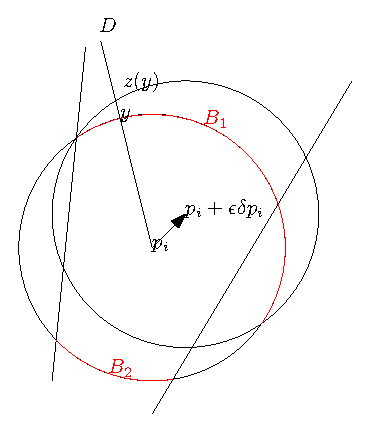
\includegraphics[scale=0.8]{2d/2d_proof_gradient_area_1}
    \caption{Situation for a ball $ B(p_i, r) $ in 2D}
    \label{fig:demo-gradient}
\end{figure}

Then, we have: $ A_\epsilon = A_0 + Vol(A_1^\epsilon) - Vol(A_2^\epsilon) +
O(\epsilon^2) $
% TODO

Now, we will approximate $ Vol(A_1^\epsilon) $ write that $ Vol(A_1^\epsilon) =
\int_{B_1} || x - z(x) || dx + o(||\delta p_i||) $. We do the same things for $
A_2^\epsilon $.

For any $ x \in B $, we define $ z(x) $ as the intersection of the half-line $ D
$ with the circle of center $ p_i + \epsilon \delta p_i $ of radius $ r $. We
also parametrize the half-line $ D $ by: $ x + t \frac{x - p_i}{||x - p_i||} $
where $ t \ge 0 $.

Let us find this intersection point by assuming that $ t $ is small
such that $ t^2 = t \delta p_i = o(||\delta p_i||^2) $.

We need to find $ D \cap C(p_i + \delta p_i, r) $. Let $ t \ge 0 $ then , we have :
\begin{equation}
    || x + t \frac{x - p_i}{||x - p_i||} - (p_i + \epsilon \delta p_i) ||^2 = r^2
    \tag{$\star$}
\end{equation}

If we expand this expression, we get:

\begin{align*}
    (\star) & \iff || x - (p_i + \epsilon \delta p_i) ||^2 + t^2 + 2t \left(
        \frac{x-p_i}{|| x - p_i||} | x - (p_i + \epsilon \delta p_i) \right) = r^2 \\
    & \iff || x - p_i || ^2 - 2 \epsilon (x - p_i | \delta p_i) + || \epsilon \delta p_i || ^2 + t^2 + 2t
    \left( \frac{x-p_i}{|| x - p_i||} | x - (p_i + \epsilon \delta p_i) \right) = r^2 \\
    & \iff -2 \epsilon (x - p_i | \delta p_i) + 2t || x - p_i|| + o(||\delta p_i||^2) = 0
    \text{ because } || x - p_i || = r \\
    & \iff t = t^{\star} = \epsilon \left( \frac{x - p_i}{||x - p_i||} | \delta p_i \right) +
    o(||\delta p_i||^2)
\end{align*}

Then, $ z(y) = x + t^{\star} \frac{x - p_i}{||x - p_i||} $ and $ || x - z(x) || =
t^{\star} $.

We deduce that :
$$ Vol(A_1^\epsilon) = \int_{B_1} \left[ \epsilon \left( \frac{x - p_i}{||x - p_i||} | \delta p_i \right) +
o(||\delta p_i||^2) \right] dx $$

And:

$$ Vol(A_1^\epsilon) - Vol(A_2^\epsilon) = \int_{B} \left[ \epsilon \left( \frac{x - p_i}{||x - p_i||} | \delta p_i \right)
+ o(||\delta p_i||^2) \right] dx $$

Finally, we have, by linearity:
$$ \nabla_{p_i} A = \int_{B} \frac{x - p_i}{||x - p_i||} dx $$

\end{proof}

Now, we will relate the previously computed gradients to the mean curvature
vector of an hypersurface.

If we suppose that we have a point cloud that is an $\epsilon$-sampling of a
smooth hypersurface $ S $, then the following proposition gives the link between
the gradient of volume of an offset of $ S $ and the mean curvature vector.

\begin{proposition}
    \label{prop:gradient-mean-curvature}
    Given an $\epsilon$-sampling $ P $ of a smooth ($ C^{\infty} $) hypersurface
    $ S $ and $ r \ge 0 $ such that: $ \epsilon \leq r \leq reach(M) $, then:
    $$ || \nabla_p A - \vec{\kappa}(p) || \leq TODO $$
    Consequently, when $ \epsilon $ and $ \frac{\epsilon}{r} $ vanish then
    $ \nabla_p A $ converges towards the mean curvature vector of $ S $ at $ p $.
\end{proposition}

To prove that, we will need two lemmas extracted from \cite{amenta1999surface}
which will tell us how the Voronoi cells look:
\begin{lemma}
    If $ S $ is an hypersurface, $ P $ an $\epsilon$-sampling of $ S $ and $ p
    \in P $, then:
    $$ V(p, P) \cap S \subseteq B\left(p, \frac{\epsilon}{1 - \epsilon}
        LFS(p)\right) $$
\end{lemma}

\begin{lemma}
    If $ S $ is an hypersurface, $ P $ an $\epsilon$-sampling of $ S $, $ p
    \in P $ and $ v \in V(p, P) $ such that $ d(p, v) \ge \nu LFS(p) $ for $ \nu
    > 0 $, then the angle at $ s $ between the vector $ v $ and the normal at
    the surface (oriented in the same direction) is at most $
    \arcsin(\frac{r}{\nu(1-r)}) + \arcsin(\frac{r}{(1-r)}) $.
\end{lemma}

These two lemmas tell us that the Voronoi cells are skinny (first lemma) and
long (second lemma).

\begin{proof}
We will first do two approximations on \ref{eqn:gradient_area_2d}:
\begin{enumerate}
    \item the first one is to suppose that the offset of $ S $ is close enough
        to the offset of $ P $. Using the computation done in
        \ref{prop:comp-vol-offsets}, we can say that the error made is in the
        order of $ O(\frac{\epsilon^2}{r}) $.
    \item the second one is that if the sampling is dense enough then we can
        replace $ p $ by the projection of $ x $ on $ S $: $ \forall p \in S,~x
        \in V(p, P),~p = p_S(x) + O(\epsilon) $, see figure
        \ref{fig:voronoi-cylinder}.  For this approximation to hold, it is
        necessary for the pointed out distance to be greater than $ \epsilon $
        i.e. $ r \gg \epsilon $ which means that $ \frac{\epsilon}{r} $ needs to
        vanish.
\end{enumerate}

\begin{figure}[h]
    \centering
    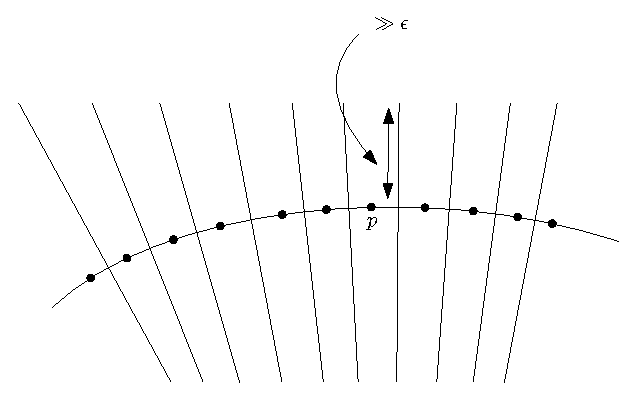
\includegraphics[scale=0.5]{img/voronoi-cylinder}
    \caption{Shape of the Voronoi cells of densely sampled points}
    \label{fig:voronoi-cylinder}
\end{figure}

Using these approximations, we get:
\begin{align*}
    \int_{\partial{P^r} \cap V(p, P)} (x - p) dx & \stackrel{(1)}{=} \int_{\partial{S^r} \cap V(p,
        P)} (x - p) dx + O(\epsilon^2) \\
    &\stackrel{(2)}{=} \int_{\partial{S^r} \cap V(p, P)} (x - p_S(x)) dx +
    O(\epsilon) \\
\end{align*}

Then, we will use the substitution $ q = p_S(x) \iff x = \phi(q) = q +
\vec{n_S}(q) $ where on the upper part of $ \partial{S^r} \cap V(p, P) $.

Using the lemma \ref{lemma:diffeo}, we have that $ \phi $ is a diffeomorphism
and that $ J_\phi(p) = (1 + \kappa_1(q)) (1 + \kappa_2(q)) $.

Using an analogous substitution on the lower part of $ \partial{S^r} \cap V(p,
P) $, we get : $ \det (D \phi) = (1 - \kappa_1(q)) (1 - \kappa_2(q)) $.

By summing the two, we obtain: $ 2 (\kappa_1(q) + \kappa_2(q)) $.

It follows that:
\begin{align*}
    \int_{\partial{S^r} \cap V(p, P)} (x - p_S(x)) dx &= \int_{S \cap V(p, P)}
    r \times \vec{n_S}(q) ( \det (id + r D \vec{n_S}(q)) - \det (id - r D
    \vec{n_S}(q)) ) dq \\
    &= 2r \int_{S \cap V(p, P)} (\kappa_1(q) + \kappa_2(q)) \vec{n_S}(q) dq \\
\end{align*}

Finally, since we have supposed that $ S $ is $ C^{\infty} $ then, we can write:
$ \vec{n_S}(q) = \vec{n_S}(p) $, $ \kappa_1(q) = \kappa_1(p) $ and $ \kappa_2(q)
= \kappa_2(p) $. All the other terms depend on the derivatives of the curvature
which are negligible at this point.

We deduce that:

$$ \nabla_p A = \partiald{A}{p} = 2r (\kappa_1(p) + \kappa_2(p)) \vec{n_S}(p)
\int_{S \cap V(p, P)} dq $$

So, using the mean curvature vector:

$$ \nabla_p A = 2r \vec{\kappa}(p) Vol(S \cap V(p, P)) $$

Which means:

$$ ||\nabla_p A - \vec{\kappa}(p) || \leq | 2r Vol(S \cap V(p, P)) - 1 |
\times|| \vec{\kappa}(p) ||$$

\end{proof}

We can summarize the situation with the following diagram:

\begin{displaymath}
    \xymatrix{A_r \ar[d]^{\nabla} \ar[r] & A \ar[d]^{\nabla} \\
        \nabla A_r \ar[r] & \nabla A }
\end{displaymath}

$ A_r $ represents the discretization of the area of an hypersurface: it
is $ \frac{Vol^d(P^r)}{2r} $ which converges towards the continuous area (see
proposition \ref{prop:approx-volume-area}). There is also a convergence property
for the gradients: the discretized gradient converges towards the continuous one
(see proposition \ref{prop:gradient-mean-curvature}).

In some sense, "discretization" and "gradient" commute: the gradient of the
discretization converges towards the continuous gradient.

% TODO

% {{{1 OTHER KINDS OF DISCRETIZATIONS
\section{Other kinds of discretizations}

% TODO: flot de l'aire du bord d'une surface = union de boules

In this work, we were also interested in other discretizations. Instead of
choosing the volume as the functional, we can also choose the area of the
boundary or corresponding weighted versions (i.e. the gradient of the volume
will be weighted by the corresponding volume of the intersection between the
Voronoi cell and a ball).

For the former case (area of the boundary), we have the following lemma:
\begin{lemma}
    If $ S $ is a smooth hypersurface whose reach is positive and $ reach(S) > r
    > 0 $, then: $$ Vol^{d-1}(S) = \frac{Vol^d(\partial S^r)}{2r} + O(r^2) $$
\end{lemma}

During this internship, we did not prove that the gradients of the area of the
boundary of a union of balls are directly connected (like for the volume of the
union) to the mean curvature of the sampled surface. But even if we did not
made the prove, we made experiments to show this relation.

Finally, we were interested in replacing the ball that we use to make the
Minkowski sum with by a convex polyhedron in order to have an anisotropic
smoothing. A more detailed study of this problem will be done in the section
dedicated to the 3D case.

% vim: set spelllang=en :
